% Options for packages loaded elsewhere
\PassOptionsToPackage{unicode}{hyperref}
\PassOptionsToPackage{hyphens}{url}
%
\documentclass[
]{book}
\usepackage{amsmath,amssymb}
\usepackage{iftex}
\ifPDFTeX
  \usepackage[T1]{fontenc}
  \usepackage[utf8]{inputenc}
  \usepackage{textcomp} % provide euro and other symbols
\else % if luatex or xetex
  \usepackage{unicode-math} % this also loads fontspec
  \defaultfontfeatures{Scale=MatchLowercase}
  \defaultfontfeatures[\rmfamily]{Ligatures=TeX,Scale=1}
\fi
\usepackage{lmodern}
\ifPDFTeX\else
  % xetex/luatex font selection
\fi
% Use upquote if available, for straight quotes in verbatim environments
\IfFileExists{upquote.sty}{\usepackage{upquote}}{}
\IfFileExists{microtype.sty}{% use microtype if available
  \usepackage[]{microtype}
  \UseMicrotypeSet[protrusion]{basicmath} % disable protrusion for tt fonts
}{}
\makeatletter
\@ifundefined{KOMAClassName}{% if non-KOMA class
  \IfFileExists{parskip.sty}{%
    \usepackage{parskip}
  }{% else
    \setlength{\parindent}{0pt}
    \setlength{\parskip}{6pt plus 2pt minus 1pt}}
}{% if KOMA class
  \KOMAoptions{parskip=half}}
\makeatother
\usepackage{xcolor}
\usepackage{longtable,booktabs,array}
\usepackage{calc} % for calculating minipage widths
% Correct order of tables after \paragraph or \subparagraph
\usepackage{etoolbox}
\makeatletter
\patchcmd\longtable{\par}{\if@noskipsec\mbox{}\fi\par}{}{}
\makeatother
% Allow footnotes in longtable head/foot
\IfFileExists{footnotehyper.sty}{\usepackage{footnotehyper}}{\usepackage{footnote}}
\makesavenoteenv{longtable}
\usepackage{graphicx}
\makeatletter
\def\maxwidth{\ifdim\Gin@nat@width>\linewidth\linewidth\else\Gin@nat@width\fi}
\def\maxheight{\ifdim\Gin@nat@height>\textheight\textheight\else\Gin@nat@height\fi}
\makeatother
% Scale images if necessary, so that they will not overflow the page
% margins by default, and it is still possible to overwrite the defaults
% using explicit options in \includegraphics[width, height, ...]{}
\setkeys{Gin}{width=\maxwidth,height=\maxheight,keepaspectratio}
% Set default figure placement to htbp
\makeatletter
\def\fps@figure{htbp}
\makeatother
\setlength{\emergencystretch}{3em} % prevent overfull lines
\providecommand{\tightlist}{%
  \setlength{\itemsep}{0pt}\setlength{\parskip}{0pt}}
\setcounter{secnumdepth}{5}
\usepackage{booktabs}
\ifLuaTeX
  \usepackage{selnolig}  % disable illegal ligatures
\fi
\usepackage[]{natbib}
\bibliographystyle{plainnat}
\usepackage{bookmark}
\IfFileExists{xurl.sty}{\usepackage{xurl}}{} % add URL line breaks if available
\urlstyle{same}
\hypersetup{
  pdftitle={Conformal Mapping},
  pdfauthor={Ashan J},
  hidelinks,
  pdfcreator={LaTeX via pandoc}}

\title{Conformal Mapping}
\author{Ashan J}
\date{2024-05-18}

\usepackage{amsthm}
\newtheorem{theorem}{Theorem}[chapter]
\newtheorem{lemma}{Lemma}[chapter]
\newtheorem{corollary}{Corollary}[chapter]
\newtheorem{proposition}{Proposition}[chapter]
\newtheorem{conjecture}{Conjecture}[chapter]
\theoremstyle{definition}
\newtheorem{definition}{Definition}[chapter]
\theoremstyle{definition}
\newtheorem{example}{Example}[chapter]
\theoremstyle{definition}
\newtheorem{exercise}{Exercise}[chapter]
\theoremstyle{definition}
\newtheorem{hypothesis}{Hypothesis}[chapter]
\theoremstyle{remark}
\newtheorem*{remark}{Remark}
\newtheorem*{solution}{Solution}
\begin{document}
\maketitle

{
\setcounter{tocdepth}{1}
\tableofcontents
}
\chapter{The Convergence Of Sequences of Analytic And Harmonic Functions}\label{the-convergence-of-sequences-of-analytic-and-harmonic-functions}

\section{The convergence of sequences of analytic functions}\label{the-convergence-of-sequences-of-analytic-functions}

Various branches of complex variable function theory, especially the geometric function theory, utilize the fundamental characteristics of converging sequences of analytic functions in their proofs. These characteristics allow for proofs that are relatively straightforward and refined compared to corresponding proofs in real analysis.

Let us give some definitions.

\begin{definition}[Point wise convergent]
\protect\hypertarget{def:unnamed-chunk-1}{}\label{def:unnamed-chunk-1}Let \(\{f_n (z)\}\), for \(n = 1, 2, \ldots\), denote a sequence of single-valued functions defined on a set \(E\) of points in the \(z\)-plane.
This sequence is said to \textbf{converge at a point \(z_0 \in E\)} if the sequence of numbers \(f_n (z_0)\) converges.
\end{definition}

\begin{definition}
\protect\hypertarget{def:unnamed-chunk-2}{}\label{def:unnamed-chunk-2}A sequence of such functions \(f_n (z)\) is said to \textbf{converge on \(E\)} if it converges at every point of \(E\).

In such a case, we may speak of the limit function \(f(z) = \lim_{n\to\infty} f_n (z)\) defined on \(E\).
\end{definition}

\begin{definition}
\protect\hypertarget{def:unnamed-chunk-3}{}\label{def:unnamed-chunk-3}The sequence \({f_n (z)}\) is said to \textbf{converge uniformly on \(E\)} to a function \(f(z)\), which is finite on \(E\), if,

\[\forall \epsilon > 0 \exists N > 0 , \forall z \in E \text{ such that } n > N \implies |f_n (z) - f(z)| < \epsilon \].
\end{definition}

\begin{definition}
\protect\hypertarget{def:unnamed-chunk-4}{}\label{def:unnamed-chunk-4}On the other hand, if \(f(z) = \infty\) on \(E\), the sequence \(f_n (z)\) is said, by definition, to \textbf{converge uniformly on \(E\) to \(\infty\)} if,
\[\forall M > 0 \exists N > 0,  \forall z \in E \text{ such that } n > N \implies |f_n (z)| > M\].
\end{definition}

\begin{definition}
\protect\hypertarget{def:unnamed-chunk-5}{}\label{def:unnamed-chunk-5}The sequence \(\{f_n(z)\}\) is a \textbf{uniform Cauchy sequence in \(E\)}, if,
\[\forall \epsilon > 0 \exists N > 0 \text{ such that } \forall z \in D, m, n > N \implies |f_n(z) - f_m(z)| < \epsilon\].
\end{definition}

\begin{proposition}
\protect\hypertarget{prp:unnamed-chunk-6}{}\label{prp:unnamed-chunk-6}Suppose that \(E \subseteq \mathbb{C}\) is a region. A sequence of complex valued functions \(\{f_n(z)\}\) converges uniformly in \(E\) if and only if it is a uniform Cauchy sequence in \(E\).
\end{proposition}

\begin{proof}
easy

Later I will do it.
\end{proof}

If the functions \(f_n (z)\) are defined on a domain \(B\), we shall need, besides the concept of uniform convergence of a sequence in the domain \(B\), the concept of uniform convergence of a sequence in the interior of the domain \(B\).

\begin{definition}
\protect\hypertarget{def:unnamed-chunk-8}{}\label{def:unnamed-chunk-8}Let functions \(f_n (z)\) be defined on a domain \(B\). Then \(f_n(z)\) is called \textbf{uniform convergent in the interior of the domain \(B\)} if there is uniform convergence of \(|f_n (z)|\) on every closed set \(E \subseteq B\).
\end{definition}

\begin{remark}
Uniform convergence in the interior of \(B\) is a weaker requirement than uniform convergence in \(B\).
\end{remark}

\begin{definition}
\protect\hypertarget{def:unnamed-chunk-10}{}\label{def:unnamed-chunk-10}A single-valued function \(f(z)\), defined and finite on a set \(E\) not including \(\infty\), is said to be \textbf{continuous on \(E\)} if,
\[\forall z_0 \in E \forall a\epsilon > 0, \exists \delta > 0 \text { such that } z \in E \text{ and } |z - z_0| < \delta \implies |f(z) - f(z_0)| < \epsilon\].
\end{definition}

\begin{theorem}
\protect\hypertarget{thm:unnamed-chunk-11}{}\label{thm:unnamed-chunk-11}\textbf{Statement:} If a sequence \(f_n (z)\) of functions that are continuous on a set \(E\) converges uniformly to a finite function \(f(z)\) defined on \(E\), this function \(f(z)\) is also continuous on \(E\).
\end{theorem}

\begin{proof}
To see this, let \(z_0 \in E\). Then, since \(f_n(z)\) is unifromaly continous, for given \(\epsilon > 0\), there exists a number \(n\) such that, for all \(z \in E\), we have \(|f_n (z) - f(z)| < \frac{\epsilon}{3}\).

Furthermore, since \(f_n(z)\) is continuous, there exists a number \(\delta > 0\) such that, for all \(z \in E\) satisfying the inequality \(|z - z_0| < \delta\), we have \(|f_n (z) - f_n (z_0)| < \frac{\epsilon}{3}\) (because of the continuity of \(f_n (z)\) on \(E\)). Therefore, for \(z \in E\) and \(|z - z_0| < \delta\), we have

\[
|f(z)-f(z_0)| \leq |f(z)- f_n (z)| + |f_n (z) - f_n (z_0)| + |f_n (z_0) -f(z_0)| < \epsilon,
\]

which means that \(f(z)\) is continuous at the point \(z_0 \in E\). It then follows that, if the functions \(f_n (z)\) are continuous in the domain \(B\) and if a sequence of them converges in the interior of \(B\) to a finite function \(f(z)\), then \(f(z)\) is continuous in \(B\).
\end{proof}

\chapter{UNIVALENT MAPPING OF MULTIPLY CONNECTED DOMAINS}\label{univalent-mapping-of-multiply-connected-domains}

\section{Univalent conformal mapping of a doubly connected domain onto an annulus}\label{univalent-conformal-mapping-of-a-doubly-connected-domain-onto-an-annulus}

\subsection{page 206}\label{page-206}

Let us now begin with the simplest case of the problem posed, namely, the
case of doubly connected domains. Let us show that every doubly connected
domain can be mapped univalently onto some circular annulus, whose boundary
circles may degenerate to points.

Let \(B\) denote a doubly connected domain in the \(z\)-plane.

If it has an isolated boundary point \(z_0\), then, by adjoining it to the domain \(B\), we obtain a simply connected domain that we can then map univalently either onto the disk \(I (I < I)\) or onto the \((-\)plane with the point \((= \infty)\) excluded. We can do this in such a way that the point \(z = z_0\) is mapped into \((= 0)\). The domain \(B\) is thus univalently mapped either onto the annulus \(0 < |z| < I\) or onto the annulus \(0 < |z| < \infty\).

Suppose now that the boundary of the domain \(B\) consists of two continua \(K_1\) and \(K_2\). One of these, let us say \(K_1\) is necessarily bounded. The complement of \(K_1\) in the \(z\)-plane is an open set consisting of two disjoint domains. One of these domains, let us say \(B_1\) contains the domain \(B\). The domain \(B_1\) is simply connected. Therefore, it can be mapped conformally onto the disk \(|z'| < I\). Under this mapping, the continuum \(K_2\) is mapped into a continuum \(K\) contained in \(|z' | < I\), and the domain \(B\) is mapped into a domain \(B'\).

Let us now map whichever of the simply connected domains complementary to \(K\) contains \(B'\) onto the domain \(|z''| > I\) in such a way that \(z' = \infty\) is mapped into \(z'' = \infty\). Under this mapping, the circle \(|z'| = I\) is mapped into an analytic Jordan curve contained in the domain \(|z''| > I\) and the domain \(B'\) is mapped into a doubly connected domain \(B''\) that does not include \(\infty\) and that is bounded by this curve and by the circle \(|z''| = I\).

The composite of these two mappings constitutes a univalent mapping of the domain \(B\) onto the domain \(B''\). Furthermore, on the basis of \(\S 3\) of Chapter II, we conclude that this mapping sets up a one-to-one correspondence between the prime ends of the domain \(B\) and the boundary points of the domain \(B''\). Here, just as in \(\S 3\) of Chapter II, by the prime end of the domain \(B\) that corresponds to the point \(z\) on the boundary of the domain \(B''\), we mean the set of all cluster points of all sequences of points of the domain \(B\) that approach the boundary point \(z\).

\chapter{Conformal Mappings}\label{conformal-mappings}

\begin{definition}[Tanagent Vector]
\protect\hypertarget{def:unnamed-chunk-13}{}\label{def:unnamed-chunk-13}Let \(\gamma(t) = x(t) + iy(t), 0\leq  t \leq  1\), be a smooth parameterized curve terminating at \(z_0 = \gamma(0)\). We refer to
\[\gamma'(0) = \lim_{t \to 0} \frac{\gamma(t)-\gamma(0)}{t} = x'(0) + iy'(0)\]
as the tangent vector to the curve 'Y at ZOo
\end{definition}

\begin{definition}[Angle between two curves ]
\protect\hypertarget{def:unnamed-chunk-14}{}\label{def:unnamed-chunk-14}We define the angle between two curves
at \(z_0\) to be the angle between their tangent vectors at \(z_O\).
\end{definition}

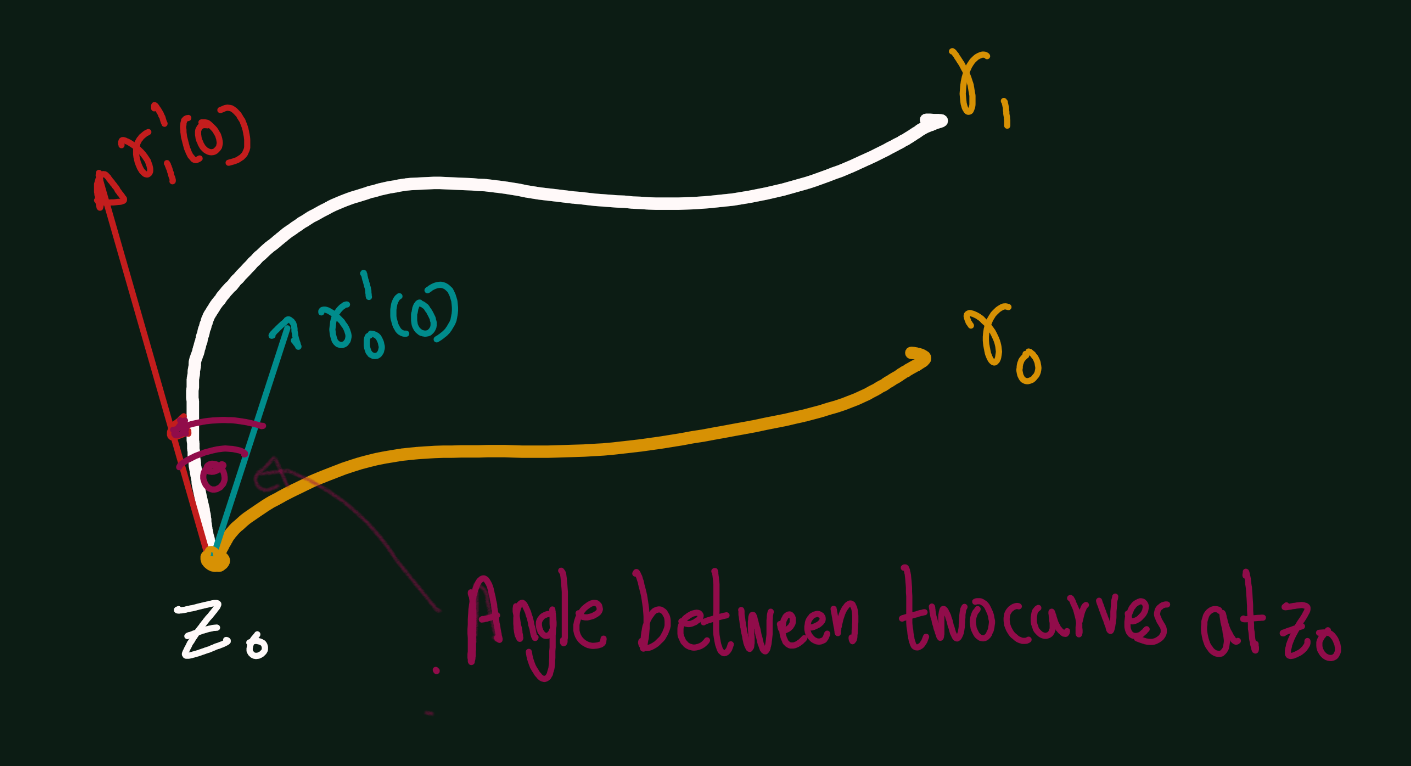
\includegraphics{figures/Confromal_mapping/fig1.png}

\begin{theorem}
\protect\hypertarget{thm:unnamed-chunk-16}{}\label{thm:unnamed-chunk-16}If \(\gamma(t)\), \(0 \leq t \leq 1\), is a smooth parameterized curve terminating at \(z_0 = \gamma(0)\), and \(f(z)\) is analytic at \(z_0\), then the tangent to the curve \(f(\gamma(t))\) terminating at \(f(z_0)\) is given by:
\begin{equation}
(f \circ \gamma)'(0) = f'(z_0)\gamma'(0)
\end{equation}
\end{theorem}

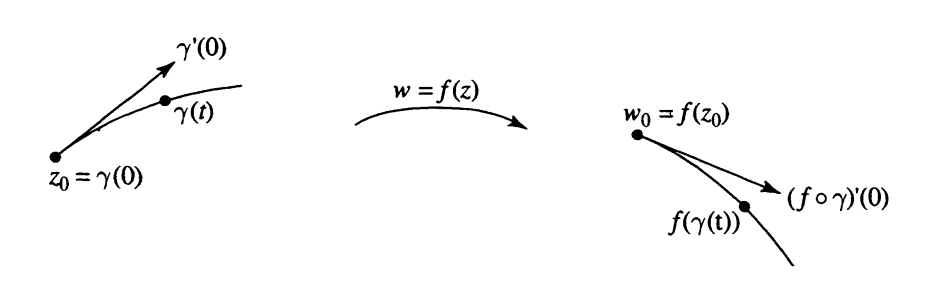
\includegraphics{figures/Confromal_mapping/fig2.png}

\begin{proof}
\leavevmode

\begin{itemize}
\tightlist
\item
  If \(\gamma'(0) \neq 0\), then \(\gamma(t) \neq \gamma(0)\) for \(t\) near \(0\), \(t \neq 0\), so we may write
  \begin{equation}
  \frac{f(\gamma(t)) - f(\gamma(0))}{t} = \frac{f(\gamma(t)) - f(\gamma(0))}{\gamma(t) - \gamma(0)} \cdot \frac{\gamma(t) - \gamma(0)}{t}
  \end{equation}
  and pass to the limit, to obtain the formula (6.1).
\item
  If \(\gamma'(0) = 0\), then proceeding as in Section 2, we obtain \((f \circ \gamma)'(0) = 0\), and again the formula holds.
\end{itemize}

\end{proof}

\chapter{Uniformization by square domains}\label{uniformization-by-square-domains}

\begin{definition}[Domain]
\protect\hypertarget{def:unnamed-chunk-19}{}\label{def:unnamed-chunk-19}A subset \(D\) of the complex plane is a domain if \(D\) is open and if any two points of \(D\) can be connected by a broken line segment in \(D\).
\end{definition}

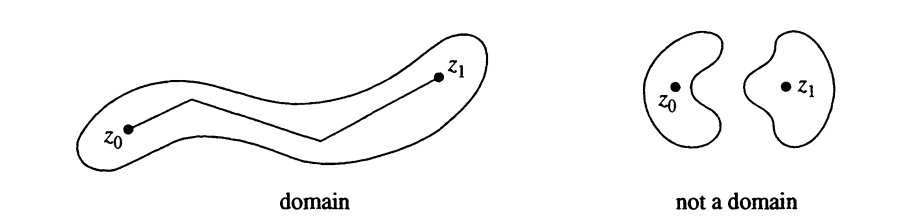
\includegraphics{figures/Mario_Bonk/fig1.png}

\begin{example}
\protect\hypertarget{exm:unnamed-chunk-21}{}\label{exm:unnamed-chunk-21}\leavevmode

\begin{itemize}
\tightlist
\item
  \textbf{Examples}:

  \begin{itemize}
  \tightlist
  \item
    Open half planes
  \item
    Open disks
  \item
    Open sectors
  \item
    Open annuli,
  \item
    Open punctured disks.
  \end{itemize}
\item
  \textbf{Non Examples}:

  \begin{itemize}
  \tightlist
  \item
    Union of the open upper and lower half-planes \(=U = \mathbb{C}\setminus\mathbb{R}\).\\
    (It is impossible to connect a point in the upper half-plane to a point in the lower half-plane by a broken line segment that does not cross the real line. )
  \end{itemize}
\end{itemize}

\end{example}

\begin{definition}[Riemann Sphere]
\protect\hypertarget{def:unnamed-chunk-22}{}\label{def:unnamed-chunk-22}The Riemann sphere, also called the extended complex plane consist of the complex numbers \(\mathbb{C}\) together with \(\infty\). The set of extended complex numbers may be written as \(\mathbb{C} \cup \{\infty\}\).
\end{definition}

\textbf{Notation}: \(\hat{\mathbb{C}}=\mathbb{C} \cup \{\infty\}\)

\begin{center}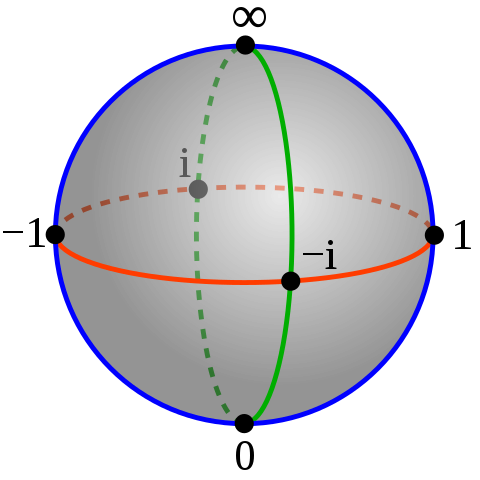
\includegraphics[height=0.5\textheight]{figures/Mario_Bonk/fig2} \end{center}

\begin{definition}
\protect\hypertarget{def:unnamed-chunk-24}{}\label{def:unnamed-chunk-24}A domain in the plane is ``simply connected'' if it has no ``holes.''
\end{definition}

\begin{example}
\protect\hypertarget{exm:unnamed-chunk-25}{}\label{exm:unnamed-chunk-25}\leavevmode

\begin{itemize}
\tightlist
\item
  \textbf{Example}

  \begin{itemize}
  \tightlist
  \item
    Disks
  \item
    Rectangles
  \end{itemize}
\item
  *\textbf{Non Example}

  \begin{itemize}
  \tightlist
  \item
    Annuli
  \item
    Punctured disks
  \item
    Punctured plane\\
    (Becasue they have ``holes'')
  \end{itemize}
\end{itemize}

\end{example}

Later we discuss this more precise

\begin{definition}[Meromophic]
\protect\hypertarget{def:unnamed-chunk-26}{}\label{def:unnamed-chunk-26}A function \(f(z)\) is meromorphic on a domain \(D\) if \(f(z)\) is analytic on \(D\) except possibly at isolated singularities, each of which is a pole.
\end{definition}

\begin{proof}
(Proof of Therom 1.1 in th paper)\\
Let \(\Omega\) be a finitely connected domain in \(\hat{\mathbb{C}}\) with \(\infty\in \Omega\) It is a known fact that there exists a conformal map \(g\) of \(\Omega\) onto a square domain \(\tilde{\Omega}\) with the normalization
\[g(z) = z + \frac{b_1}{z} + \ldots\]
near \(\infty\).

The map \(f \in \mathcal{F} \mapsto \tilde{f} := f \circ g^{-1}\) is a bijection between \(\mathcal{F}\) and \(\tilde{\mathcal{F}}\). Moreover, if
\[f(z) = z + \frac{a_1}{z} + \ldots ~\text{ and } \tilde{f}(z) = z + \frac{\tilde{a_1}}{z} + \ldots\] near \(\infty\), then \(\tilde{a}_1 = a_1 - b_1\).
\end{proof}

Let \(f\) be as in the statement. We consider the rectangle \(R = [-l,l] \times [-r,r] \subset \mathbb{C}\) for large \(r > 0\). Here we chose \(l= = r^{2/3}\) so that
\[ \frac{l}{r} \to  0 \quad \text{and} \quad \frac{r}{l^2} \to 0\]
as \(r \to \infty\).

In the following, we assume that \(r\) is so large that \(\widetilde{C}\setminus \Omega\) is contained in the interior of \(R\). Then \(\partial R \subset \widetilde{C}\setminus \Omega\) and \(j=f(R)\) is a Jordan curve in \(\mathbb{C}\). We want to

\begin{eqnarray}
A &=& \frac{1}{2i} \int_J \bar{w} dw\\
&=& \frac{1}{2i} \int_{\partial R} \bar{f(z)}f'(z) dz\\
&=& \frac{1}{2i} \int_{\partial R} \overline{\left(z + \frac{a_1}{z} + \ldots \right)} \left(1 - \frac{a_1}{z^2} + \ldots \right) dz\\
&=& \frac{1}{2i} \int_{\partial R} \left(\bar{z} + \frac{\bar{a}_1}{\overline{z}}-\frac{\bar{a}_1\bar{z}}{z^2} + O\left(\frac{1}{|z|^2}\right)\right) dz\\
&=& 4rl + \int_{\partial R} \text{Im} \left(\frac{\bar{a}_1 z}{\bar{z}}\right) \frac{dz}{z} + o(1).
\end{eqnarray}

Sure, I can provide a proof for the proposition. Here it goes:

\textbf{Proposition}: If a set \(A\) is a subset of the interior of another set \(B\) (denoted as \(A \subseteq Int(B)\)), then the complement of \(A\) (denoted as \(A^c\)) is a subset of the boundary of \(B\) (denoted as \(bd(B)\)).

\textbf{Proof}:

Let's denote the interior of \(B\) as \(Int(B)\) and the boundary of \(B\) as \(bd(B)\). By definition, we have:

\begin{enumerate}
\def\labelenumi{\arabic{enumi}.}
\tightlist
\item
  \(Int(B) = B - bd(B)\)
\item
  \(A^c = U - A\) where \(U\) is the universal set.
\end{enumerate}

Given that \(A \subseteq Int(B)\), we can say that \(A\) does not contain any points from \(bd(B)\). Therefore, all points in \(bd(B)\) must be in \(A^c\).

Hence, \(A^c \subseteq bd(B)\).

This completes the proof. Please note that this is a general proof and the specifics might vary depending on the exact definitions and properties of the sets and the topological space they are in. If you have a specific example or further questions, feel free to ask!

\chapter{Riemann Mapping Theorem}\label{riemann-mapping-theorem}

\begin{theorem}[Riemann Mapping Theorem]
\protect\hypertarget{thm:unnamed-chunk-28}{}\label{thm:unnamed-chunk-28}If \(D\) is a simply connected domain in the complex plane, and \(D\) is not the entire complex plane, then there is a conformal map of \(D\) onto the open unit disk \(\mathbb{D}\).
\end{theorem}

\section{Hyperbolic Geomeery}\label{hyperbolic-geomeery}

Suppose \(w = f(z)\) is a conformal self-map of the open unit disk \(\mathbb{D}\). From Pick's lemma we then have equality,
\[\left|\frac{d\omega}{dz}\right|=\frac{1-|\omega|^2}{1-|z|^2}\]
In differential form this becomes
\[\frac{|dw|}{1-|w|^2} = \frac{|dz|}{1-|z|^2},\]
which means that if \(\gamma\) is any smooth curve in \(\mathbb{D}\), and \(\omega=f(z)\) is a conformal self-map of \(\mathbb{D}\), then
\[\int_{f\circ \gamma}\frac{|dw|}{1-|w|^2} =\int_{\gamma} \frac{|dz|}{1-|z|^2}.\]
Thus to obtain a length function that is invariant under conformal self-maps of \(\mathbb{D}\),we are led to make the following definition. We define the
length of \(\gamma\) in the hyperbolic metric by
\[\text{hyperbolic length of } \gamma = =\int_{\gamma} \frac{|dz|}{1-|z|^2}\]

\section{Proof of Riemann Mapping Theorem}\label{proof-of-riemann-mapping-theorem}

Recall the following theorem.

\begin{theorem}
\protect\hypertarget{thm:thm1}{}\label{thm:thm1}

The following properties are equivalent, for a domain \(D\) in the complex plane:

\begin{enumerate}
\def\labelenumi{\roman{enumi}.}
\tightlist
\item
  \(D\) is simply connected,
\item
  every closed differential on \(D\) is exact,
\item
  for each \(z_0 \in \mathbb{C} \setminus D\), there is an analytic branch of \(\log(z - z_0)\) defined
  on \(D\),
\item
  each closed curve \(\gamma\) in \(D\) has winding number \(W(\gamma, z_0) = 0\) about all points \(z_0 \in \mathbb{C} \setminus D\),
\end{enumerate}

\begin{enumerate}
\def\labelenumi{(\alph{enumi})}
\setcounter{enumi}{21}
\tightlist
\item
  the complement of \(D\) in the extended complex plane \(\hat{\mathbb{C}}\) is connected.
\end{enumerate}

\end{theorem}

Suppose that \(D\) is simply connected and that \(D \neq \mathbb{C}\). Choose \(a \in \mathbb{C} \setminus D\). By the characterization of simple connectivity,
By theorem \ref{thm:thm1}, there is an analytic branch \(g(z)\) of \(\log(z - a)\) in \(D\).
Then,
\[h(z) = e^{g(z)/2}=e^{\left(\frac{log(z-a)}{2}\right)}=(z-a)^{\frac{1}{2}}=\sqrt{z-a}\]
So, \(h(z) = e^{g(z)/2}\) is an analytic branch of \(\sqrt{z - a}\) in \(D\), and \((h(z))^2 = z - a \neq 0\) (Since \(a\not\in D\)) in \(D\). If \(h(z_1) = h(z_2)\), then \[z_1 = (h(z_1))^2 + a = (h(z_2))^2 + a = z_2\].
Thus \(h(z)\) is univalent, and \(h(z)\) maps \(D\) conformally onto \(h(D)\). Finally, note that if \(w_0 \in h(D)\), then \(-w_0 \notin h(D)\). Indeed, if \(w_0 = h(z_0)\) and \(-w_0 = h(z_1)\) for \(z_0, z_1 \in D\), then \(z_0 = h(z_0)^2 + a = w_0^2 + a = h(z_1)^2 + a = z_1\), which is impossible. We summarize.

\begin{lemma}
\protect\hypertarget{lem:unnamed-chunk-29}{}\label{lem:unnamed-chunk-29}Let \(D\) be a simply connected domain. Suppose \(a \notin D\), and let
\(h(z)\) be an analytic branch of \(\sqrt{z - a}\) in \(D\). Then \(h(z)\) is univalent on \(D\), and further, \(h(D)\) is disjoint from \(-h(D)\).
\end{lemma}

\begin{proof}
Done it earler.
\end{proof}

  \bibliography{book.bib,packages.bib}

\end{document}
